
\documentclass[11pt]{article}
\usepackage[margin=0.9in]{geometry}
\usepackage{xeCJK}
\usepackage{amsmath,amssymb}
\usepackage{graphicx,booktabs,array,hyperref,float}
\setCJKmainfont{PingFang SC}
\setlength{\emergencystretch}{3em}

\title{MAT3300 Final Project --- Problem C\\[2pt]
\large Question 6: How one genre evolves --- the jazz influence process, 1930s--2000s}
\author{虞紫涵 (Yu Zihan)\\Student ID: 123090773\\The Chinese University of Hong Kong, Shenzhen}
\date{}

\begin{document}
\maketitle

\section{The question, the data, and the choice of jazz}
The sixth task asks us to analyse the influence process of musical evolution over time in
\emph{one} genre, to identify indicators that reveal the dynamic influencers, and to explain how
the genre and its artists changed. We take jazz as the genre. The choice continues Question~1:
the Jazz-induced influence subnetwork already described in Question~1
(384 artists, 1,769 edges) spans the whole record, and it gives
the analysis a well-documented internal history --- swing, bebop, cool jazz, hard bop, free jazz,
fusion, crossover --- against which the data-driven periods can be read.

The data are the same four files and the same cleaning as Question~1, with Assumption~A3 of the
joint report: all 42,770 reported pairs are retained, including the 733 time-order reversals.
Of the 5,603 artists in the influence network, 406 carry the Jazz label as
their main genre; they are involved in 3,073 influence edges, of which
1,769 have jazz at both ends.
The Spotify files contain 8,000 songs by 404 of these artists; 285
artists have at least three songs and can be given a stable feature vector.
Table~\ref{tab:data} collects the counts.

\begin{table}[!ht]
\centering
\small
\begin{tabular}{lr}
\toprule
Quantity & Value \\
\midrule
Raw influence records & 42,770 \\
Influence edges retained (Assumption A3) & 42,770 \\
Time-order reversals retained & 733 \\
Same-decade edges & 8,477 \\
Artists in the influence network & 5,603 \\
Edges with at least one jazz endpoint & 3,073 \\
Jazz$\to$jazz edges & 1,769 \\
Artists in the jazz influence subnetwork & 384 \\
Artists labelled Jazz & 406 \\
Jazz artists with at least 3 songs & 285 \\
Jazz songs & 8,000 \\
Artists with at least one jazz song & 404 \\
Song years & 1924--2020 \\
Yearly timeline (years with $\ge 20$ songs) & 1936--2002 \\
Jazz$\to$jazz pairs used for transmission & 937 \\
Artists with a usable transmission score & 175 \\
Artists with at least 5 jazz followers & 59 \\
\bottomrule
\end{tabular}
\caption{Jazz data used in this section. The influence network is the cleaned network of
Question~1; the song features are the per-song entries of \texttt{full\_music\_data.csv}.}
\label{tab:data}
\end{table}

Two properties of the source data shape the design.
First, \texttt{data\_by\_artist} gives one career average per artist, not a time series.
We therefore work at the song level: every song is compared with the sound of jazz in its own
release year, and the artist's deviation is the average of these song-level deviations.
Second, \texttt{active\_start} is a decade, so the artist's position on the timeline is
decade-coarse; we use it only to place the artist's generation, never to date individual songs.

\section{A sonic timeline for jazz}
\subsection{The feature space}
We use the nine continuous audio features of the data (danceability, energy, valence, tempo,
loudness, acousticness, instrumentalness, speechiness, and duration), with duration on a
logarithmic scale, each standardised against the 5,854 artists of \texttt{data\_by\_artist.csv}.
A value of $+1$ therefore means one population standard deviation above the average recording of
the whole corpus, not of jazz.
We exclude \texttt{liveness}. On these records it mostly separates live albums from studio albums:
a $k$-means run that includes it sets apart a 589-song cluster almost entirely by
liveness ($+4.7$ standard deviations), which is a recording artefact rather than a style.
Mode and key are categorical and are not used.

The genre's timeline is the yearly mean feature vector $m(y)$ over jazz songs, computed for years
with at least 20 songs, smoothed with a centred three-year window and linearly interpolated
between years.
This leaves a reliable yearly series from 1936 to 2002; earlier and later years remain
in the decade summaries but not in the yearly velocity curve.

\subsection{The decade trajectory}
Table~\ref{tab:decades} and Figure~\ref{fig:timeline} summarise the movement.
The most acoustic decade is the 1930s (acousticness 0.91, duration 3.0 minutes, tempo 124~BPM);
the 1970s is the most electric and the longest (acousticness 0.48, duration 6.7 minutes, energy
0.51); the 1980s--2000s return part way towards an acoustic, quieter sound without returning to the
1930s values.

\begin{table}[!ht]
\centering
\small
\begin{tabular}{crcccccc}
\toprule
Decade & Songs & Acoustic. & Energy & Tempo & Valence & Instrum. & Duration \\
 & & & & (BPM) & & & (min) \\
\midrule
1930s & 149 & 0.91 & 0.30 & 124 & 0.62 & 0.44 & 3.0 \\
1940s & 235 & 0.89 & 0.33 & 119 & 0.55 & 0.48 & 3.7 \\
1950s & 3,652 & 0.79 & 0.30 & 113 & 0.50 & 0.36 & 4.9 \\
1960s & 2,409 & 0.74 & 0.30 & 111 & 0.45 & 0.37 & 5.6 \\
1970s & 633 & 0.48 & 0.51 & 115 & 0.55 & 0.47 & 6.7 \\
1980s & 460 & 0.55 & 0.39 & 112 & 0.49 & 0.38 & 5.3 \\
1990s & 295 & 0.60 & 0.37 & 113 & 0.46 & 0.33 & 4.9 \\
2000s & 135 & 0.57 & 0.44 & 110 & 0.47 & 0.37 & 4.8 \\
\bottomrule
\end{tabular}
\caption{Raw decade centroids of jazz songs. ``Acoustic.'', ``Energy'', ``Valence'' and
``Instrum.'' are Spotify features on their original scales; duration is in minutes.}
\label{tab:decades}
\end{table}

A principal-component analysis of the yearly centroids makes the shape of the trajectory
explicit (Figure~\ref{fig:timeline}a).
The first component explains 59.3\% of the variance and loads positively on acousticness and
negatively on duration (duration $-0.79$, acousticness $+0.52$, energy $-0.24$): it separates short acoustic recordings from long electric
ones.
The second component explains 16.8\% and loads on instrumentalness $+0.58$, energy $+0.48$, valence $+0.42$.
The 1930s and 1940s sit at the acoustic, short end; the 1950s and 1960s move left as tracks
lengthen and darken; the 1970s jump far to the electric, loud, long corner; the 1980s--2000s
return towards the middle.
The trajectory is a loop rather than a line: jazz modernised and then partly re-acousticised,
and a one-dimensional ``more modern'' axis would miss the reversal.

\begin{figure}[!ht]
\centering
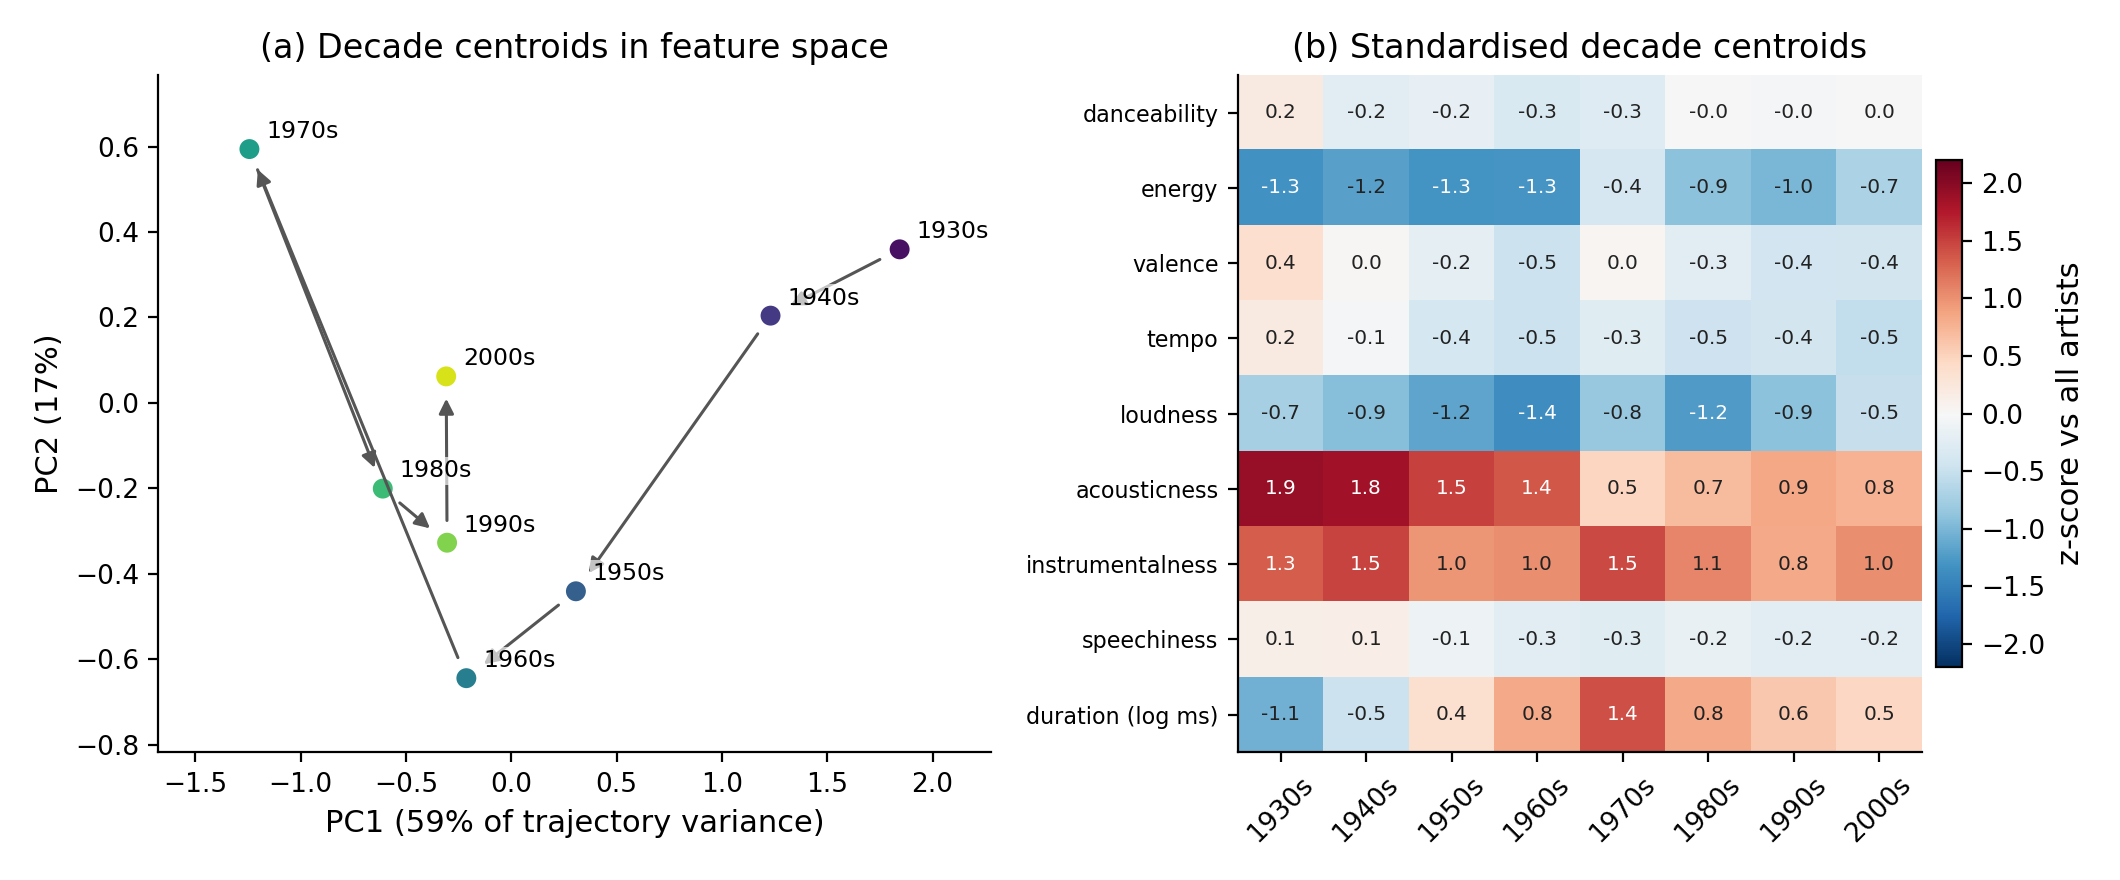
\includegraphics[width=\linewidth]{figures/fig1_genre_timeline.png}
\caption{(a) Decade centroids of jazz in the space of the first two principal components of the
yearly centroids; arrows follow the decades. (b) Standardised decade centroids of the nine
features (z-scores against all 5,854 artists).}
\label{fig:timeline}
\end{figure}

\subsection{Episodes of rapid change}
The velocity of the centroid, $\|m(y+2)-m(y-2)\|$ in z-units, measures how fast the genre's sound
moved. Figure~\ref{fig:revolutions}a shows four well-separated local maxima, at 1949, 1954, 1969 and 1980.
The feature decomposition of each episode (Figure~\ref{fig:revolutions}b and
Table~\ref{tab:episodes}) identifies what kind of change each one was.

\begin{table}[!ht]
\centering
\small
\begin{tabular}{clp{0.62\linewidth}}
\toprule
Year & Speed & Largest feature changes (z-units, $y-2\to y+2$) \\
\midrule
1949 & 2.23 & duration $-1.28$, loudness $-1.07$, energy $-1.00$, speechiness $-0.84$ \\
1954 & 1.65 & duration $+1.58$, instrumentalness $-0.43$, valence $-0.18$, energy $-0.09$ \\
1969 & 1.23 & duration $+0.76$, energy $+0.56$, acousticness $-0.55$, loudness $+0.48$ \\
1980 & 1.19 & speechiness $+0.59$, loudness $-0.51$, valence $-0.51$, energy $-0.47$ \\
\bottomrule
\end{tabular}
\caption{The four episodes of rapid centroid movement and the features that moved most.}
\label{tab:episodes}
\end{table}

The episodes are not all stylistic.
The 1949 episode is the break with the swing baseline: recordings become shorter, quieter, less
energetic and less speech-like, the profile of the small bebop group after the big band.
The 1954 episode is dominated by duration ($+1.58$ z, with the next largest change,
instrumentalness, at $-0.43$): this is consistent with the LP replacing the 78-rpm single, a
format change that allowed long performances.
The 1969 episode is the electric turn --- acousticness falls by 0.55 z while energy, loudness and
duration rise --- and the 1980 episode is a quieter, more acoustic, more speech-like production,
consistent with the crossover and smooth-jazz turn together with the beginning of the acoustic
revival.
A definition of ``revolution'' that looked only at style would miss the format revolution of the
1950s; the feature decomposition separates them.

\begin{figure}[!ht]
\centering
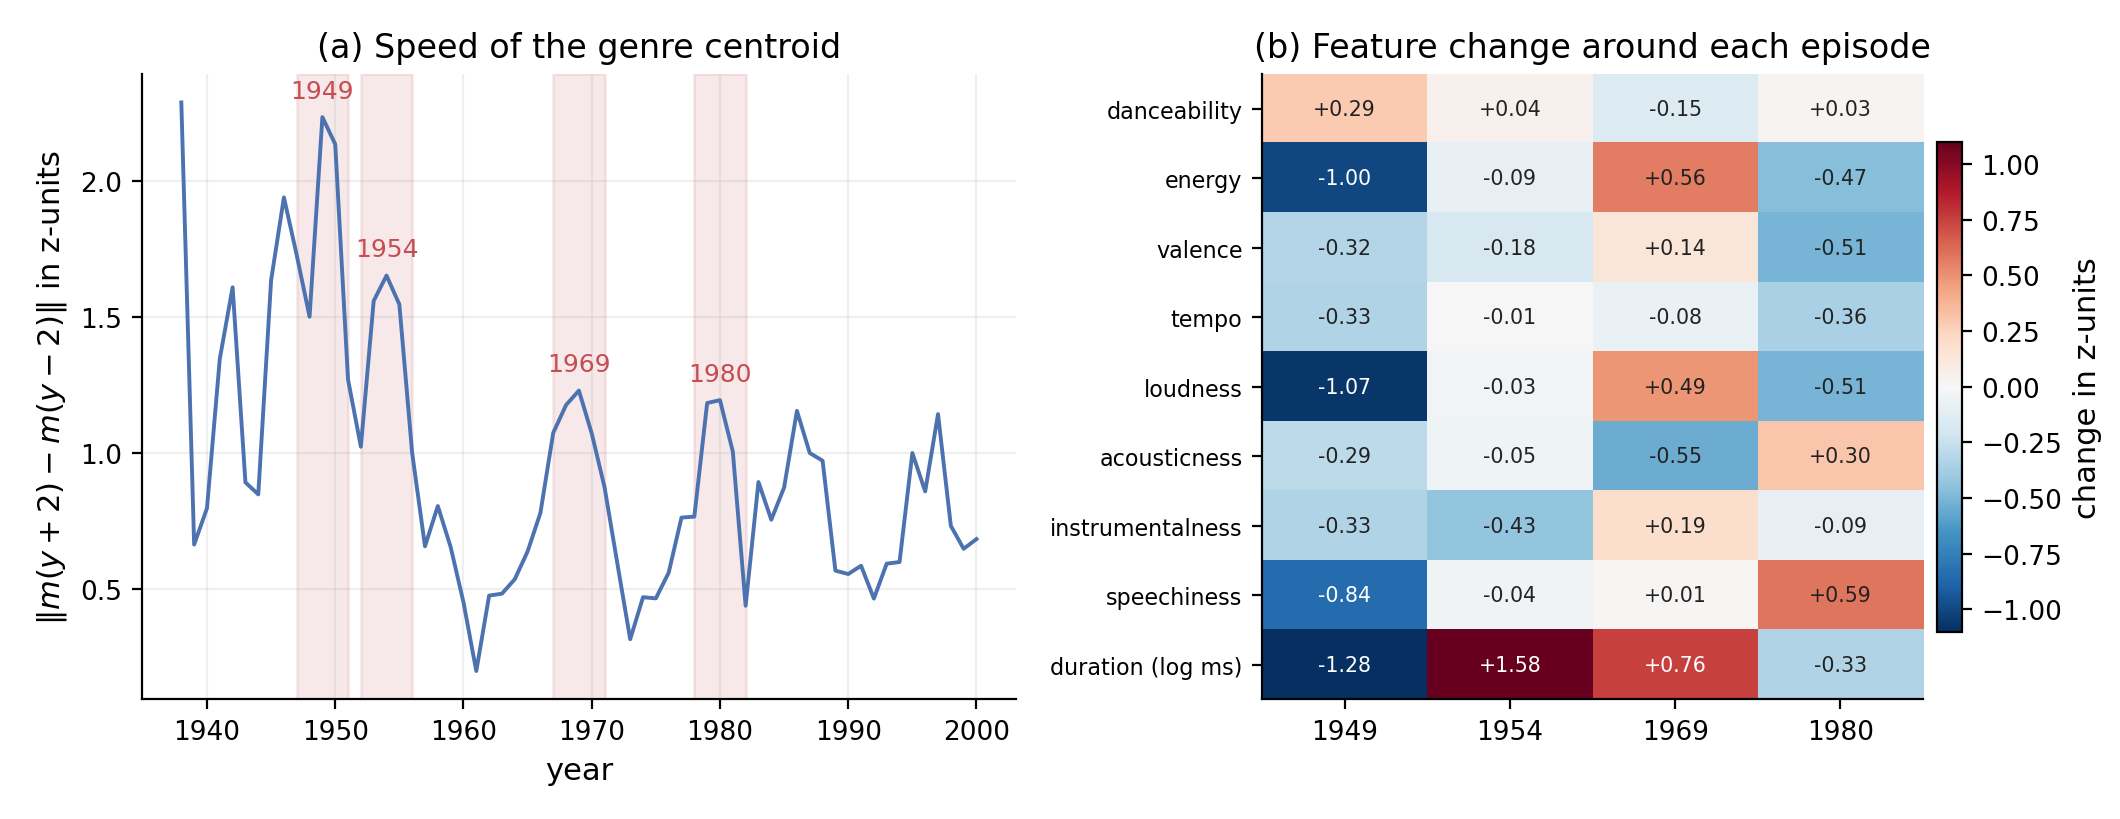
\includegraphics[width=\linewidth]{figures/fig2_revolutions.png}
\caption{(a) Speed of the jazz centroid; shaded bands mark the four episodes. (b) Change in each
feature around each episode, $m(y+2)-m(y-2)$ in z-units.}
\label{fig:revolutions}
\end{figure}

\section{Indicators of dynamic influence}
\subsection{Definitions}
For artist $i$ with at least three songs, let
\[
r_i=\frac{1}{n_i}\sum_{s\in i}\bigl(z_s-m(y_s)\bigr)
\]
be the artist's \emph{time-adjusted deviation}: the average of the song vectors, each centred on
the jazz centroid of its release year.
Four indicators are built from $r_i$ and from the influence edges.

\paragraph{Originality $N_i$.}
$N_i=\|r_i\|_\Sigma$, the Mahalanobis length of the deviation using the covariance of the 5,854
artist vectors. It measures how far the artist's sound was from the jazz of their own time, in
units that account for the correlations among features.

\paragraph{Anticipation $A_i$.}
Let $t_i$ be the artist's active-start decade and
$\Delta_i=m(t_i+10)-m(t_i)$ the direction in which the genre moved over the following ten years.
Then
\[
A_i=\cos\bigl(r_i,\Delta_i\bigr)\in[-1,1].
\]
A positive $A_i$ means that the artist's deviation from their own generation pointed where the
genre was about to go; a negative value means the opposite. The score is undefined for artists who
started in 2000 or later, because the timeline has no reliable ten-year future; for the 1930s
cohort the first reliable centroid (1936) is used as the starting point.

\paragraph{Transmission $H_i$.}
For each jazz$\to$jazz edge $i\to j$ with $t_j>t_i$ and at least three songs for both artists, compute
$\cos(r_j,r_i)$, the alignment of the follower's deviation with the influencer's deviation, and
average over the followers of $i$. Because many artists have few followers, we report the shrunk
value
\[
H_i^*=H_i\,\frac{n_i^H}{n_i^H+3},
\]
which pulls small samples towards zero. $H_i^*$ asks whether the people who name $i$ actually
moved their music in $i$'s direction.

\paragraph{Reach.}
$K_i$ is the out-going Katz centrality of $i$ inside the Jazz-induced subnetwork, with the same
attenuation $\alpha=0.1$ as Question~1; $B_i$ is the number of non-jazz artists who name $i$.
$K$ measures reach inside the genre and $B$ measures reach across its boundary.

The sonic indicators are computed on 283 artists with a defined anticipation score;
175 of them have a usable transmission score and 59 have at least five jazz
followers.
No indicator uses popularity or any label other than ``is this artist jazz''.

\subsection{Validation: is the reported influence visible in the followers' music?}
There are 937 jazz$\to$jazz pairs with a later follower and at least three songs for both
artists.
The mean alignment is 0.164.
The permutation null reassigns each follower to a random jazz artist of the same active-start
decade, which preserves the decade composition of the pairs but destroys the reported edges.
Over 2,000 draws the null mean is 0.024 with standard deviation 0.030 (99th
percentile 0.093), and the observed value gives $p<0.001$; the bootstrap 95\%
confidence interval for the mean is $[0.105,\,0.222]$.
56.4\% of the real pairs have a positive alignment, against 51.2\% in the null.

The effect is real but modest: the reported influence is a noisy signal, not a deterministic
transfer, and the test controls for decade composition but not for shared scene, label, or
geography.
It supports the weaker claim that is actually needed here: on average, the artists who are named as
influences are the artists in whose direction their followers' music moves.

\subsection{The indicators are not redundant}
The Spearman correlations among the indicators are small (Figure~\ref{fig:validation}b):
originality and anticipation correlate $-0.02$, originality and Katz $-0.37$,
anticipation and Katz $+0.11$, and transmission and Katz $+0.25$.
Originality is negatively related to citation ($-0.35$ with future followers), while
anticipation and transmission are weakly positive ($+0.09$ and $+0.29$).
The most novel artists are not the most cited ones, and being ahead of the genre is nearly
independent of being central in it.
The indicators therefore measure different things, which is what makes the typology below useful.

\begin{figure}[!ht]
\centering
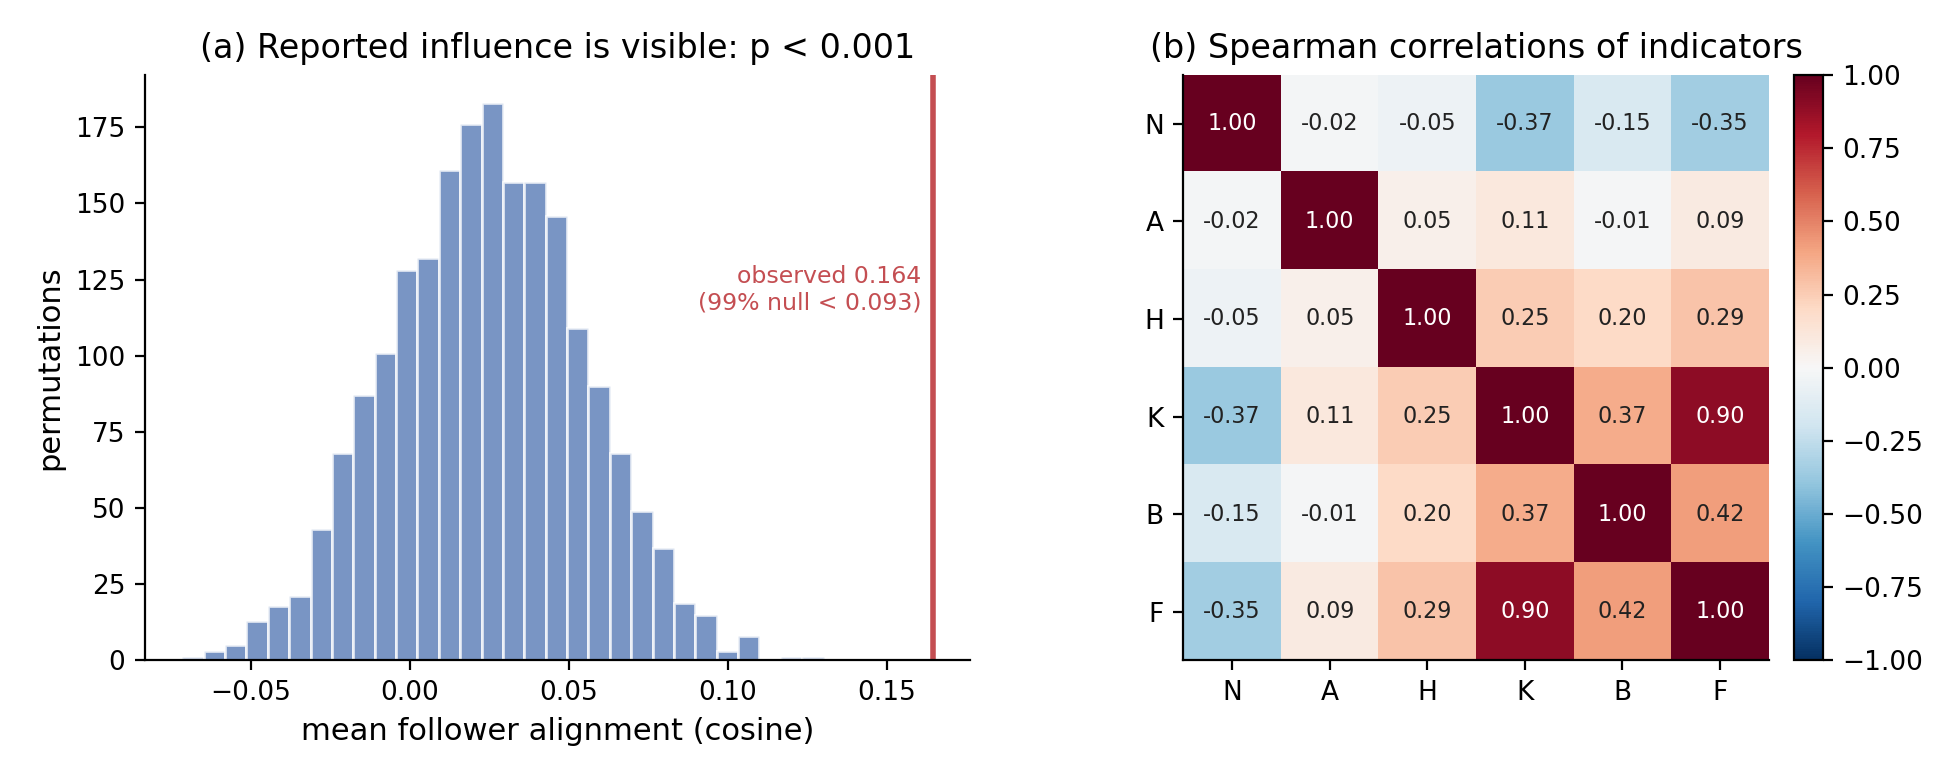
\includegraphics[width=0.95\linewidth]{figures/fig4_validation.png}
\caption{(a) Permutation null for the mean follower alignment with the observed value.
(b) Spearman correlations among originality $N$, anticipation $A$, transmission $H^*$, within-jazz
Katz $K$, boundary reach $B$, and future followers $F$.}
\label{fig:validation}
\end{figure}

\section{Who the indicators reveal}
\subsection{Four roles}
Combining the indicators separates four roles that a single centrality ranking cannot distinguish
(Table~\ref{tab:roles}).
The \emph{canon} has high within-genre Katz: Charlie Parker, Lester Young, Miles Davis, Dizzy
Gillespie, Thelonious Monk and John Coltrane.
Their anticipation scores are mixed and often negative, because they define the centre of their
generation rather than deviate from it.
The \emph{catalysts} have both high anticipation and high transmission: Dave Brubeck, George Duke,
Tal Farlow, Grover Washington, Jr., David Sanborn and Bob James.
Their sound pointed where jazz went, and their followers moved with them.
The \emph{prophets} are ahead of their time but were not copied in their own direction; the table
lists Duke Jordan, Shelly Manne, Jimmy Giuffre and John Lewis, and the same pattern appears for
Herbie Hancock, Lee Morgan and Andrew Hill.
The \emph{bridges} export influence beyond jazz: Miles Davis (77 non-jazz followers), Nat King Cole
(52), John Coltrane (52), Quincy Jones (25) and Sun Ra (24).

\begin{table}[!ht]
\centering
\small
\begin{tabular}{lp{0.17\linewidth}p{0.62\linewidth}}
\toprule
Role & Signature & Examples \\
\midrule
Canon & high $K$ & Charlie Parker (A +0.26, H* +0.03, K 17.2); Lester Young (A -0.81, H* -0.40, K 15.5); Miles Davis (A -0.33, H* +0.11, K 13.9); Dizzy Gillespie (A +0.25, H* +0.31, K 11.8) \\
Catalyst & high $A$ and high $H^*$ & Dave Brubeck (A +0.61, H* +0.62); George Duke (A +0.36, H* +0.66); Tal Farlow (A +0.92, H* +0.38); Grover Washington, Jr. (A +0.23, H* +0.70) \\
Prophet & high $A$, low $H^*$ & Duke Jordan (A +0.86, H* -0.37); Shelly Manne (A +0.85, H* -0.26); Jimmy Giuffre (A +0.82, H* -0.20); John Lewis (A +0.76, H* -0.16) \\
Bridge & high $B$ & Miles Davis (B 77); Nat King Cole (B 52); John Coltrane (B 52); Quincy Jones (B 25) \\
\bottomrule
\end{tabular}
\caption{Four roles revealed by the indicators. $A$ is anticipation, $H^*$ shrunk transmission,
$K$ within-jazz Katz, $B$ non-jazz followers.}
\label{tab:roles}
\end{table}

\subsection{The dynamic influencers}
We rank artists by the dynamic-influence score
\[
S_i=z(A_i)+z(H_i^*),
\]
the equal-weight sum of the two standardised sonic indicators.
Table~\ref{tab:top} gives the top twelve among the 59 artists with at least five jazz
followers; ranks are stable when the weights are changed (Spearman 0.910--0.979 for $A$ weights
from 0.3 to 0.7).

\begin{table}[!ht]
\centering
\small
\begin{tabular}{rlccccccc}
\toprule
\# & Artist & Start & $N$ & $A$ & $H^*$ & Followers & $K$ & $B$ \\
\midrule
1 & Dave Brubeck & 1940s & 1.13 & +0.61 & +0.62 & 8 & 2.13 & 6 \\
2 & George Duke & 1960s & 1.62 & +0.36 & +0.66 & 5 & 1.69 & 10 \\
3 & Tal Farlow & 1940s & 2.46 & +0.92 & +0.38 & 8 & 3.03 & 2 \\
4 & Grover Washington, Jr. & 1960s & 1.19 & +0.23 & +0.70 & 8 & 2.32 & 1 \\
5 & David Sanborn & 1960s & 1.43 & +0.76 & +0.30 & 5 & 1.76 & 0 \\
6 & Bob James & 1960s & 1.76 & +0.30 & +0.50 & 6 & 1.77 & 2 \\
7 & Barney Kessel & 1940s & 3.38 & +0.69 & +0.23 & 6 & 4.81 & 2 \\
8 & Erroll Garner & 1940s & 2.18 & +0.74 & +0.20 & 11 & 4.52 & 4 \\
9 & Nat King Cole & 1930s & 2.31 & +0.54 & +0.27 & 11 & 5.07 & 52 \\
10 & Horace Silver & 1950s & 1.64 & +0.53 & +0.26 & 11 & 5.76 & 5 \\
11 & Oscar Peterson & 1940s & 2.44 & +0.79 & +0.12 & 14 & 4.66 & 4 \\
12 & Clifford Brown & 1950s & 1.42 & +0.69 & +0.15 & 6 & 3.13 & 0 \\
\bottomrule
\end{tabular}
\caption{Top twelve dynamic influencers. $N$ originality, $A$ anticipation, $H^*$ transmission,
``Followers'' the number of usable jazz followers, $K$ within-jazz Katz, $B$ non-jazz followers.}
\label{tab:top}
\end{table}

Two groups dominate.
The first is the cool/hard-bop generation of the 1940s--50s: Brubeck, Farlow, Barney Kessel,
Erroll Garner, Oscar Peterson, Horace Silver and Clifford Brown.
The second is the crossover generation of the 1960s: George Duke, Grover Washington, Jr., David
Sanborn and Bob James.
Both are moments at which the genre's centre moved, and in both the leading artists are not the
canonical names of Table~\ref{tab:roles}.
This is the main answer to the ``dynamic influencers'' part of the question: the artists who move
a genre are not necessarily the artists with the largest citation counts.
The canon supplies continuity; the catalysts supply direction.

\begin{figure}[H]
\centering
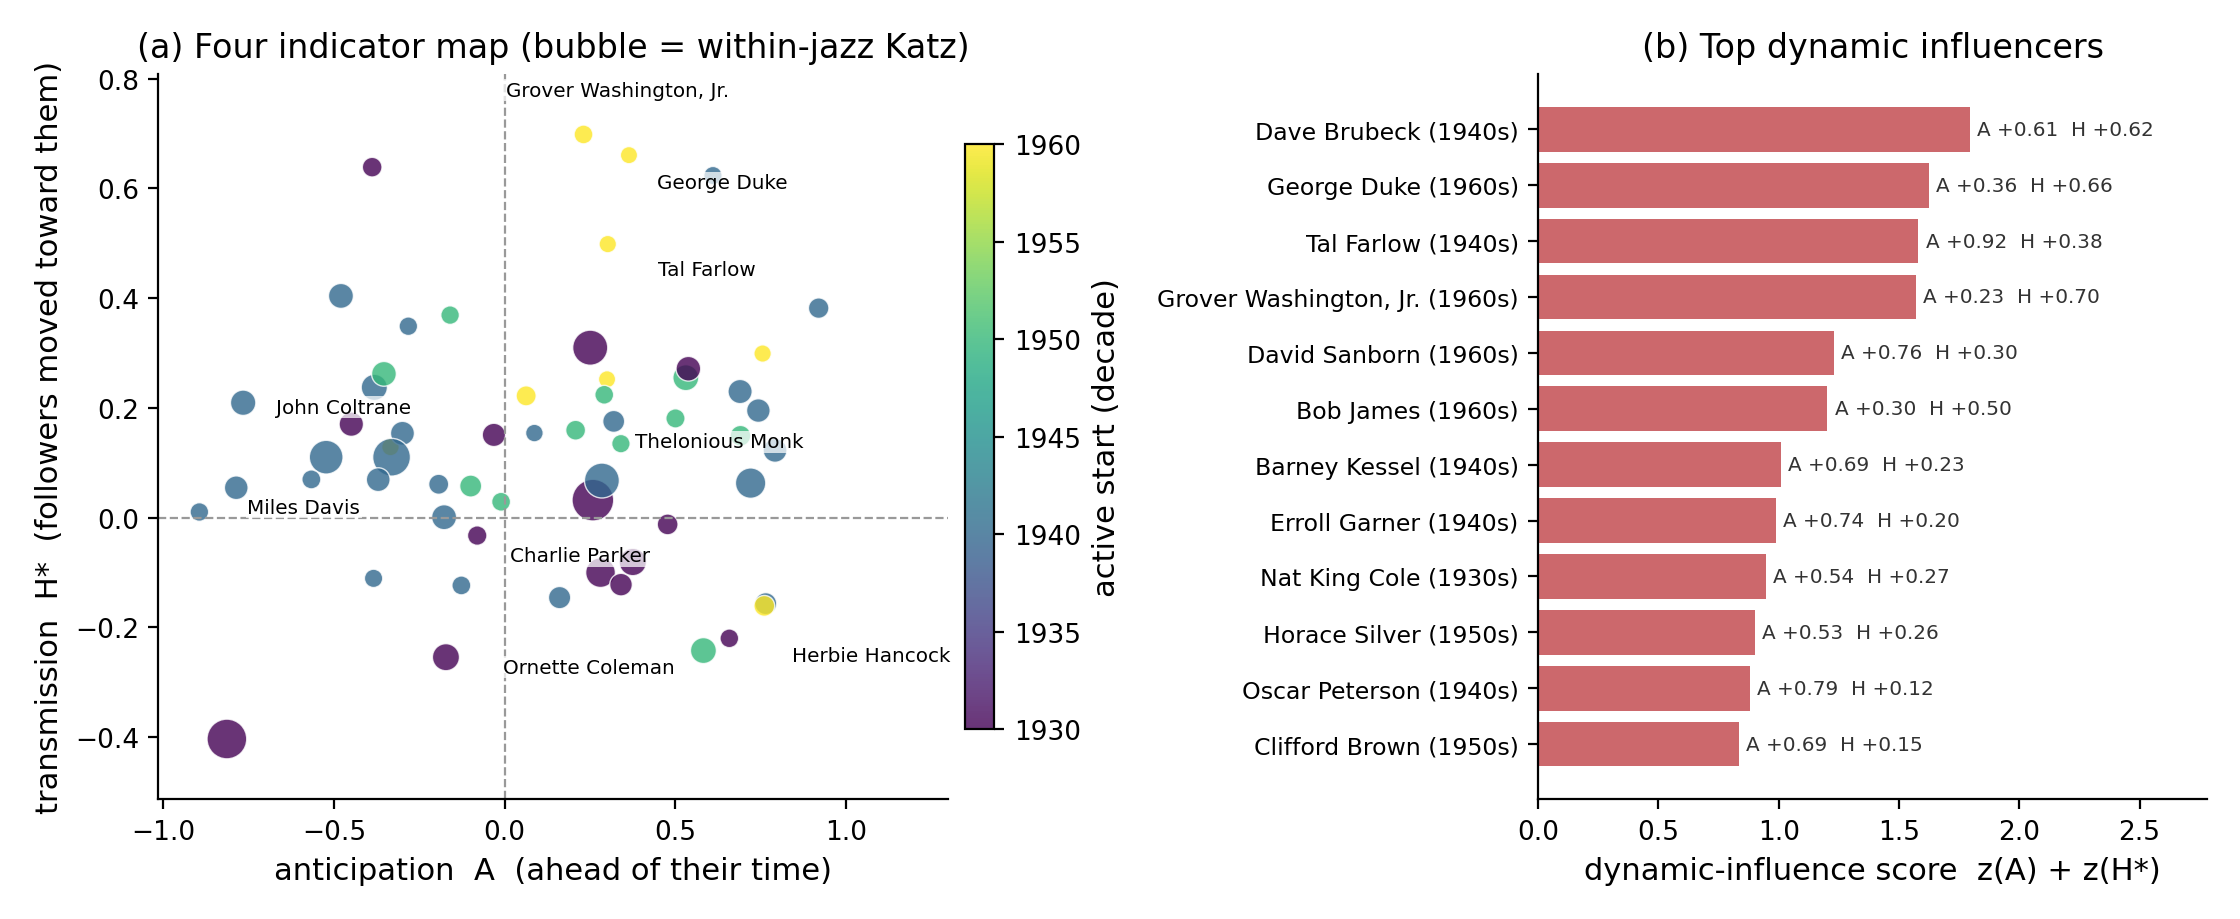
\includegraphics[width=\linewidth]{figures/fig5_influencers.png}
\caption{(a) Anticipation against transmission for artists with at least five jazz followers;
bubble area is within-jazz Katz and colour is the active-start decade. (b) The top twelve by
$S=z(A)+z(H^*)$, annotated with the two component scores.}
\label{fig:influencers}
\end{figure}

\section{How jazz changed, period by period}
The indicators and the timeline can be read together as a sequence of influence regimes.

\paragraph{1930s--mid-1940s: the swing baseline}
The decade centroid is the most acoustic and the shortest of the series (acousticness 0.91,
duration 3.0 minutes, tempo 124~BPM, valence 0.62), and the sound is dominated by up-tempo
acoustic small groups.
Lester Young is the pure canon type: within-jazz Katz 15.5, anticipation $-0.81$ and transmission
$-0.41$; his followers did not move towards his deviations, they reproduced the centre he already
defined.
Cab Calloway is a bridge (23 non-jazz followers) rather than a sonic catalyst, and Roy Eldridge is
a second, less extreme canon case.

\paragraph{Late 1940s: bebop}
The 1949 episode is the cleanest stylistic break: duration $-1.28$, energy $-1.00$, loudness
$-1.07$ and speechiness $-0.85$ z, with danceability rising.
The small group replaces the big band.
Charlie Parker has the highest within-jazz Katz (17.2) but only $A=0.26$ and $H^*=0.03$: the
revolution is visible in the cohort's shift, not in Parker's distance from it.
Bud Powell is the exception on the sonic side ($A=0.72$) and Gillespie combines a high centrality
with a positive transmission ($H^*=0.31$).

\paragraph{1950s: cool jazz, hard bop and the long-playing record}
The 1954 episode is almost entirely a duration shift ($+1.58$ z), consistent with the LP
replacing the 78-rpm single.
Tracks lengthen from 3.0 minutes in the 1930s to 4.9 minutes in the 1950s, and the 1954 episode is
the largest duration change in the series.
The dynamic influencers of this period are Brubeck ($A=0.61$, $H^*=0.62$), Farlow ($A=0.92$),
Kessel, Garner, Oscar Peterson, Horace Silver and Clifford Brown.
The Brubeck case is the clearest: a sound that was both ahead of the 1940s centre and copied by
later musicians.

\paragraph{Late 1950s--1960s: cool, modal, hard bop and the avant-garde}
The decade is darker and slower: valence falls to 0.45, the lowest of the series, and acousticness
to 0.75.
The canon and the avant-garde separate.
Coltrane and Miles remain central ($K=10.8$ and $13.9$) but have negative anticipation
($-0.52$ and $-0.33$): they are the centre, not ahead of it.
Ornette Coleman ($A=0.58$, $H^*=-0.24$, 16 non-jazz followers), Cecil Taylor ($A=0.81$, only two
usable jazz followers), Herbie Hancock ($A=0.76$, $H^*=-0.16$) and Andrew Hill ($A=0.70$,
$H^*=-0.31$) are the ahead-of-time group; their influence is either absorbed later or exported
rather than copied directly within the genre.

\paragraph{Late 1960s--1970s: fusion}
The 1969 episode is the electric turn (acousticness $-0.55$, energy $+0.56$, loudness $+0.48$,
duration $+0.76$).
The 1970s centroid is the most electric (acousticness 0.48), the highest-energy (0.51) and the
longest (6.7 minutes), the average track length being the highest of any decade.
Hancock ($A=0.76$), Tony Williams ($A=0.73$), John McLaughlin ($A=0.39$, $H^*=0.48$, five non-jazz
followers) and Weather Report (10 non-jazz followers) carry the change; Miles Davis is the
boundary bridge with 77 non-jazz followers.
Here the ``prophet'' and ``bridge'' roles overlap: the fusion idea travelled both inside jazz and
out of it.

\paragraph{1980s--2000s: crossover, smooth jazz and the acoustic revival}
The 1980 episode reverses several signs at once (energy $-0.47$, valence $-0.51$, acousticness
$+0.30$, speechiness $+0.59$): a quieter, more vocal, more produced sound.
Acousticness partially recovers (0.55 in the 1980s, 0.60 in the 1990s against 0.48 in the 1970s)
and the average track length falls back to 4.8 minutes by the 2000s.
The dynamic influencers are now the crossover musicians --- George Duke ($A=0.35$, $H^*=0.66$),
Grover Washington, Jr. ($A=0.23$, $H^*=0.70$), Bob James ($A=0.30$, $H^*=0.50$) and David Sanborn
($A=0.76$, $H^*=0.30$) --- while the canon remains Miles, Coltrane and Parker.
Wynton Marsalis ($A=0.31$, no usable jazz follower in this edge set) marks the neoclassical
reaction, but the data give him no transmission score.

Across the whole period the influence process has two mechanisms.
\emph{Canonical transmission} reproduces the centre: the most cited artists define what the next
generation sounds like, and the mechanism shows up as high $K$ with low $A$ and $H^*$.
\emph{Catalytic transmission} moves the centre: an artist's deviation from their generation points
where the genre goes, and their followers move towards it, which shows up as high $A$ and $H^*$.
The genre's largest moves occur when the second mechanism meets an opening that is not itself
musical --- the LP in the 1950s, electric instruments and amplification in the late 1960s, and
multitrack pop production in the 1980s.
This is also how the ``social, political or technological'' dimension of the problem enters the
network: it enters as a change in the recording format and production that shifts the feature
centroid before the influence network catches up.

\section{Robustness and limitations}
\paragraph{Leave-one-out centroids.}
Recomputing each artist's residual and anticipation with that artist's own songs removed from the
yearly centroid changes the rankings only marginally: Spearman 0.996 for originality and
0.999 for anticipation. The artist's own contribution to a centroid of several hundred songs
is too small to drive the result.

\paragraph{Shrinkage, feature set and horizon.}
The shrinkage of the transmission score is not driving the ranking: among the 59 artists
with at least five followers, raw and shrunk transmission correlate at Spearman 0.993.
Adding liveness back gives Spearman 0.965 for originality and 0.993 for anticipation.
Shortening the anticipation horizon from ten to five years gives 0.766: the ten-year horizon
matters, and the five-year version is a different, noisier question. The reported score uses the
ten-year horizon.

\paragraph{The transmission test.}
The permutation null preserves the follower's decade but not the follower's genre, because all
pairs are jazz$\to$jazz; it also does not control for shared scene or label. The observed effect is
an association between reported influence and sonic direction, not a causal effect. The positive share (56\% against 51\%) shows that the effect is a modest shift of the whole
distribution, not a few extreme pairs.

\paragraph{Coverage and measurement.}
Only 285 of the 406 jazz artists have at least three songs, and only 175 have a usable
transmission score; the 59 artists with at least five followers are the defensible
ranking set. The 2010s contain 22 jazz songs and are excluded from the decade figures; the 1920s
contain only 9. Active-start is a decade, and it comes from AllMusic while the features come from
Spotify, so an artist's generation and their recordings can be misaligned by a few years.
Career-spanning artist averages are replaced by song-level residuals, but a song's year is its
release year, not its composition year.
Finally, the genre label is coarse: ``Jazz'' covers swing, bebop, free jazz and smooth jazz, and
the sub-genre is not observed.
A $k$-means partition of the songs was also computed; its silhouette is only 0.17 and the
solution changes with small changes to the song set, so we use the continuous trajectory and the
episodes rather than hard clusters.

\section{Conclusion}
Jazz's sonic centre moved through a loop: acoustic and short in the 1930s, longer and darker
through the 1950s--60s, electric and long in the 1970s, then partly acoustic again.
Four episodes mark the largest moves, and their feature decompositions separate a stylistic
revolution (1949), a format revolution (1954), an electric revolution (1969) and a
crossover/acoustic reversal (1980).

Four indicators make the dynamic influencers visible.
Originality, anticipation, transmission and reach are nearly independent of one another, and the
transmission indicator passes a within-decade permutation test ($p<0.001$; mean alignment 0.164
against a null of 0.024).
The resulting typology separates the canon (Parker, Young, Miles, Gillespie, Monk, Coltrane) from
the catalysts (Brubeck, Farlow, Duke, Washington, Sanborn, James), the prophets (John Lewis,
Hancock, Lee Morgan, Andrew Hill) and the bridges (Miles, Nat King Cole, Coltrane, Quincy Jones,
Sun Ra).
The artists who moved jazz are not the artists with the largest citation counts: the canon supplies
continuity, while the catalysts supply direction, and the genre's largest changes occur when a
catalytic sound meets a non-musical opening such as a new recording format or a new instrument.

\paragraph{Code and reproducibility.}
\texttt{q6\_analysis.py} produces every number and figure in this section from the four problem
files; \texttt{q6\_results.json} stores the numbers used in the tables, \texttt{q6\_artists.csv}
stores the full artist-level indicator table, and \texttt{generate\_q6\_pdf.py} rebuilds this
document.

\begin{thebibliography}{9}
\bibitem{problem} 2021 ICM Problem D, \emph{The Influence of Music}, problem statement (provided).
\bibitem{allmusic} \texttt{influence\_data.csv}, influence relations scraped from AllMusic.com,
as provided in the problem data set.
\bibitem{spotify} \texttt{full\_music\_data.csv}, \texttt{data\_by\_artist.csv} and
\texttt{data\_by\_year.csv}, Spotify audio features, as provided in the problem data set.
\bibitem{katz} L. Katz, A new status index derived from sociometric analysis,
\emph{Psychometrika} 18 (1953), 39--43.
\bibitem{gioia} T. Gioia, \emph{The History of Jazz}, 3rd ed., Oxford University Press, 2021.
\bibitem{giddins} G. Giddins and S. DeVeaux, \emph{Jazz}, W. W. Norton, 2009.
\end{thebibliography}

\end{document}
